\documentclass{revtex4-2}
\usepackage{braket,amsmath,amssymb,graphicx,float,hyperref,color,ulem,soul}
\allowdisplaybreaks
\bibliographystyle{apsrev4-1}
\begin{document}
\title{Corrections to the extended-SIAM project}
\maketitle

{\bf RG equations}\par\noindent
\[\Delta U = \rho(D_0)\Delta D \left[4V^2 \left(\frac{1}{d_1} - \frac{1}{d_0}\right) - \frac{J^2}{d_2}\right] ,\quad \Delta V = -\rho(D_0)\Delta D \frac{3 V J}{8}\left(\frac{1}{d_2} + \frac{1}{d_1}\right)~,\quad \Delta J = -\rho(D_0)\Delta D \frac{ J\left(J + 4U_b\right)}{d_2}~,\]
where the denominators \(d_i\) are given by
\[d_0 = \omega - \frac{D}{2} + \frac{U_b}{2} - \frac{U}{2},~d_1 = \omega - \frac{D}{2} + \frac{U_b}{2} + \frac{U}{2} + \frac{J}{4}~, d_2 = \omega - \frac{D}{2} + \frac{U_b}{2} + \frac{J}{4}~.\]

{\bf RG flows and phase diagram}\par\noindent
\[U_0 \sim 100U_b - 130U_b,\quad \omega = -U_0/4, \quad \rho(D_0) = 1/D_0\]
\begin{figure}[htpb]
\centering
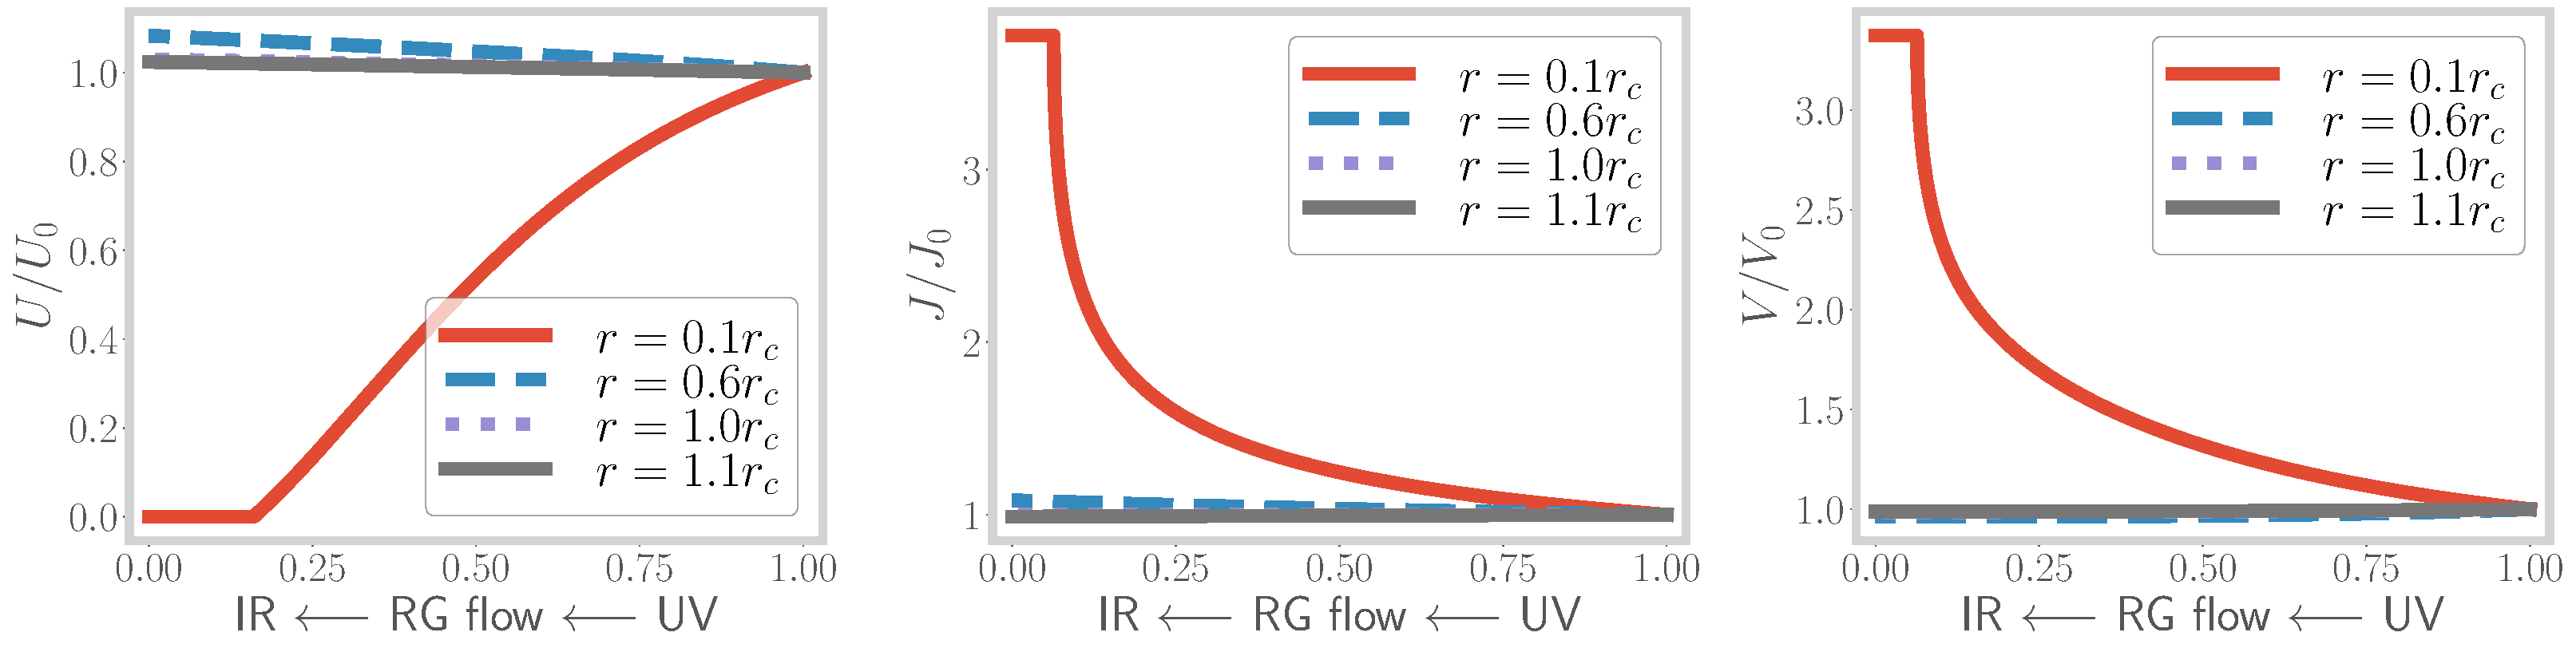
\includegraphics[width=0.8\textwidth]{rg-flows-all.pdf}
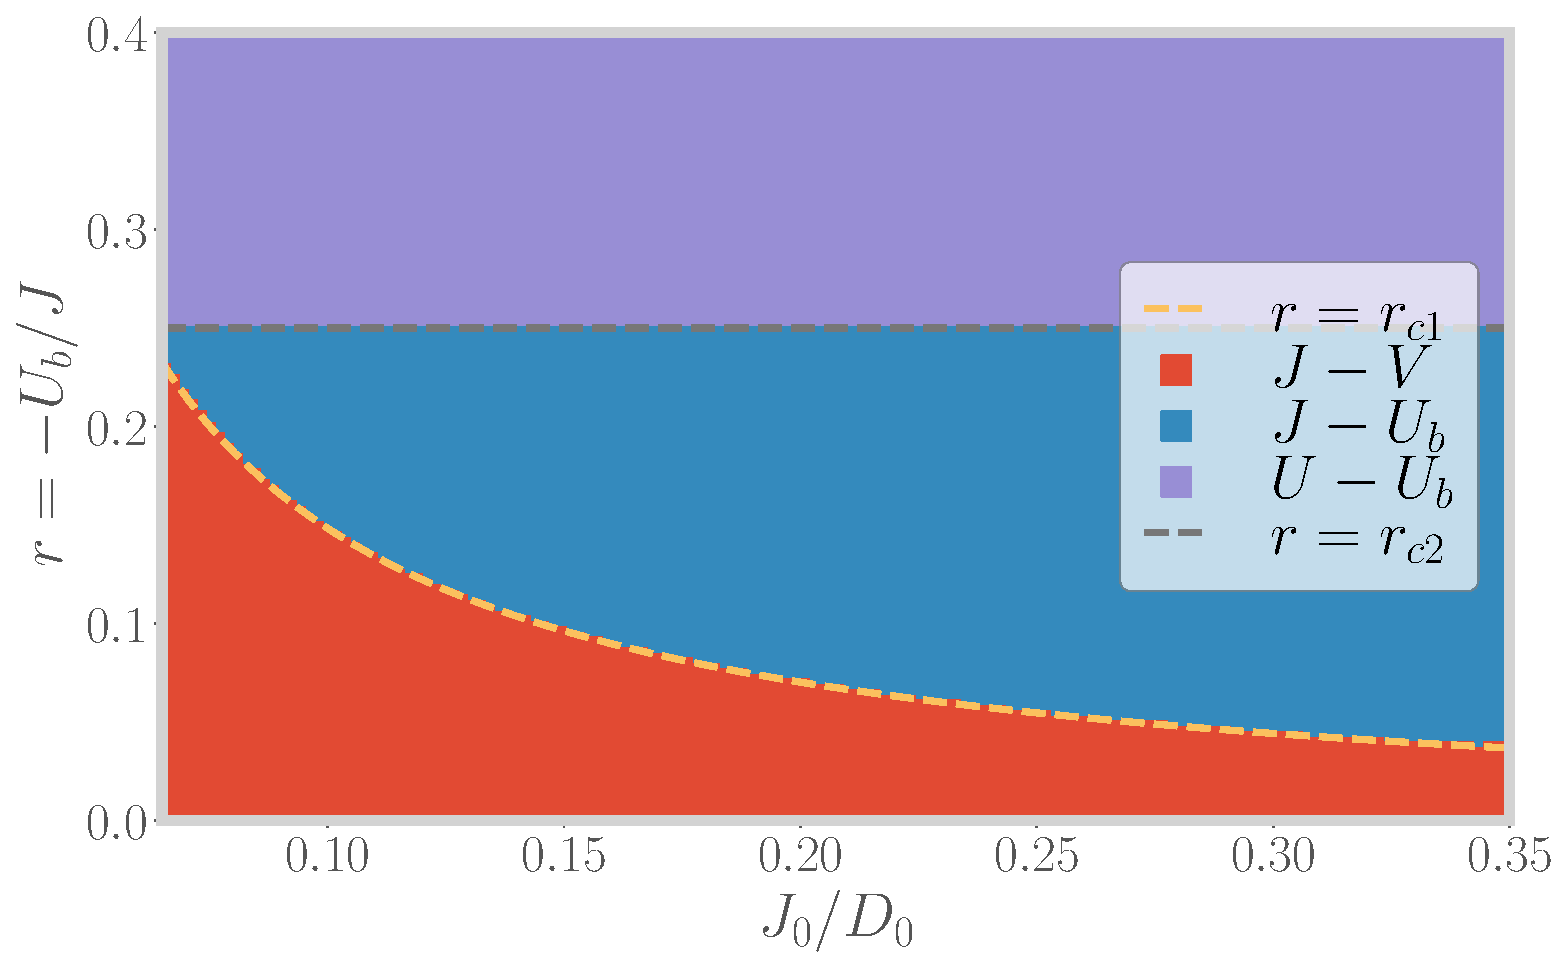
\includegraphics[width=0.5\textwidth]{phase-map-MIT.pdf}
\end{figure}

{\bf Spectral function}\par\noindent
\begin{figure}[htpb]
	\centering
	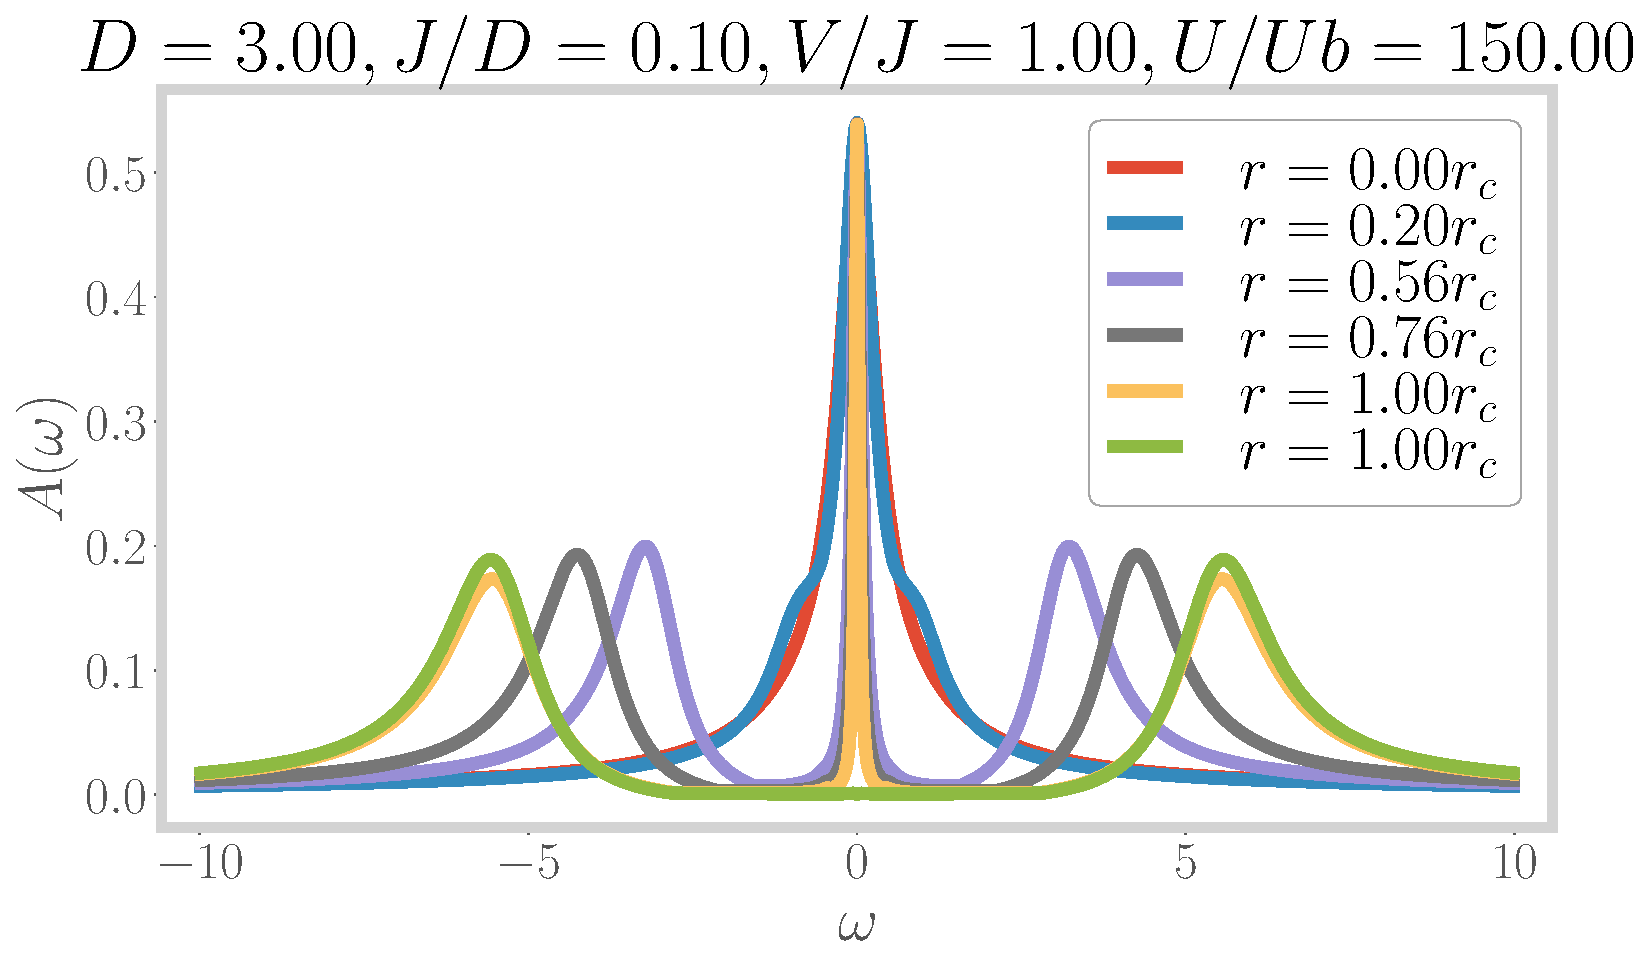
\includegraphics[width=0.5\textwidth]{spectral-function-D=3.00_J_by_D=0.10_V_by_J=1.00_U_by_Ub=150.00.pdf}
\end{figure}

{\bf Correlations across full range}\par\noindent
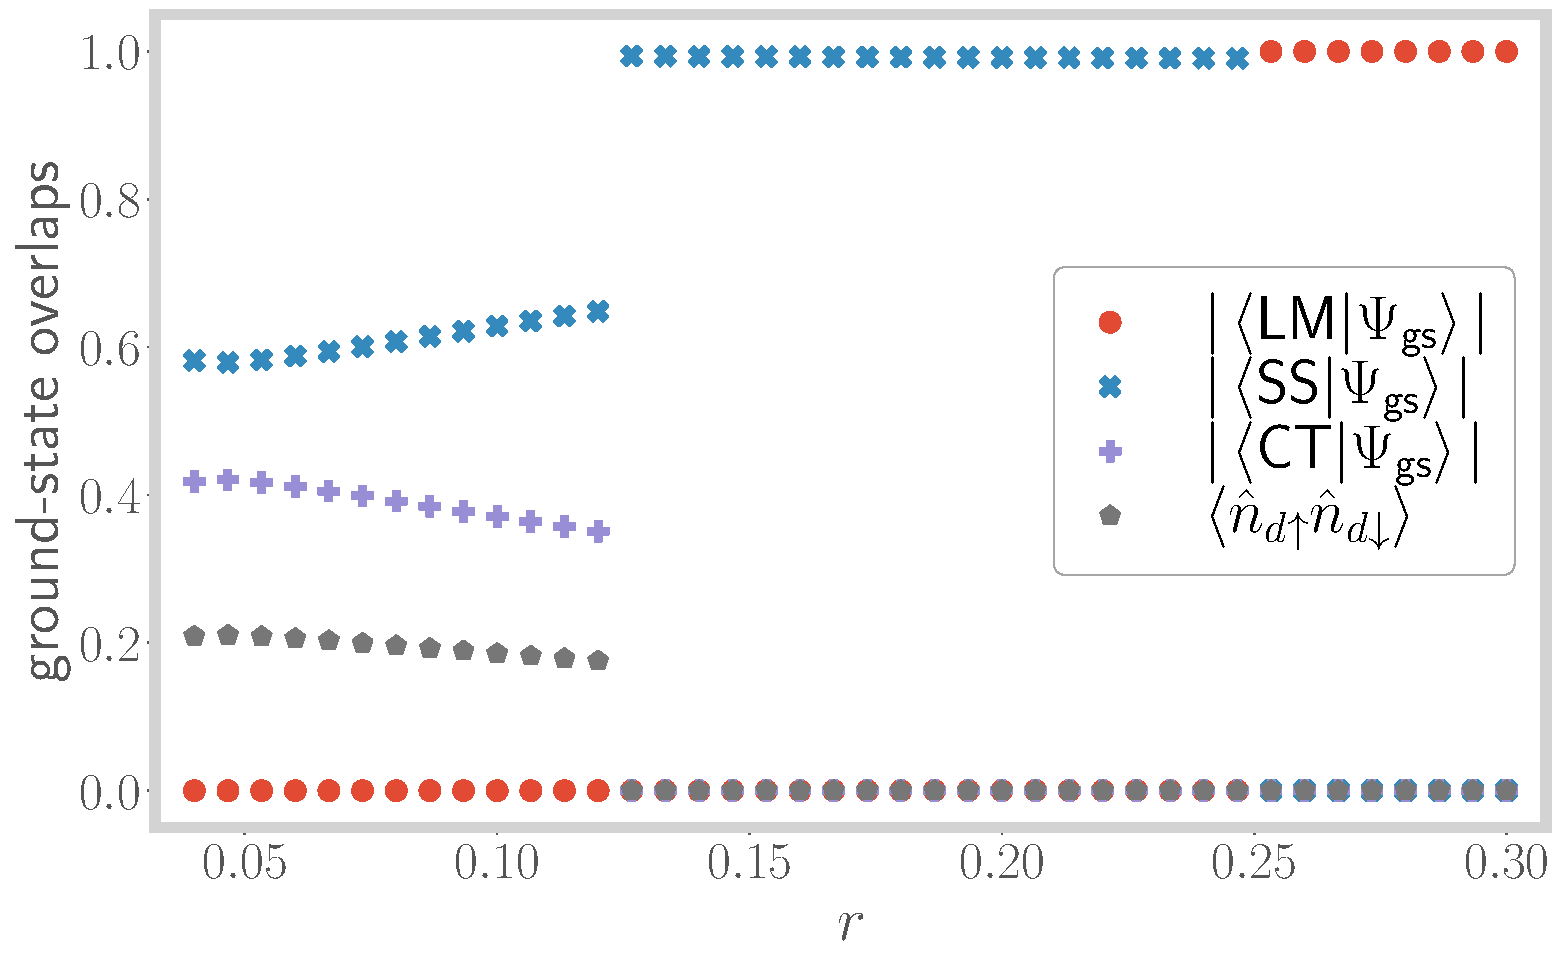
\includegraphics[width=0.4\textwidth]{corrs_gs.pdf}
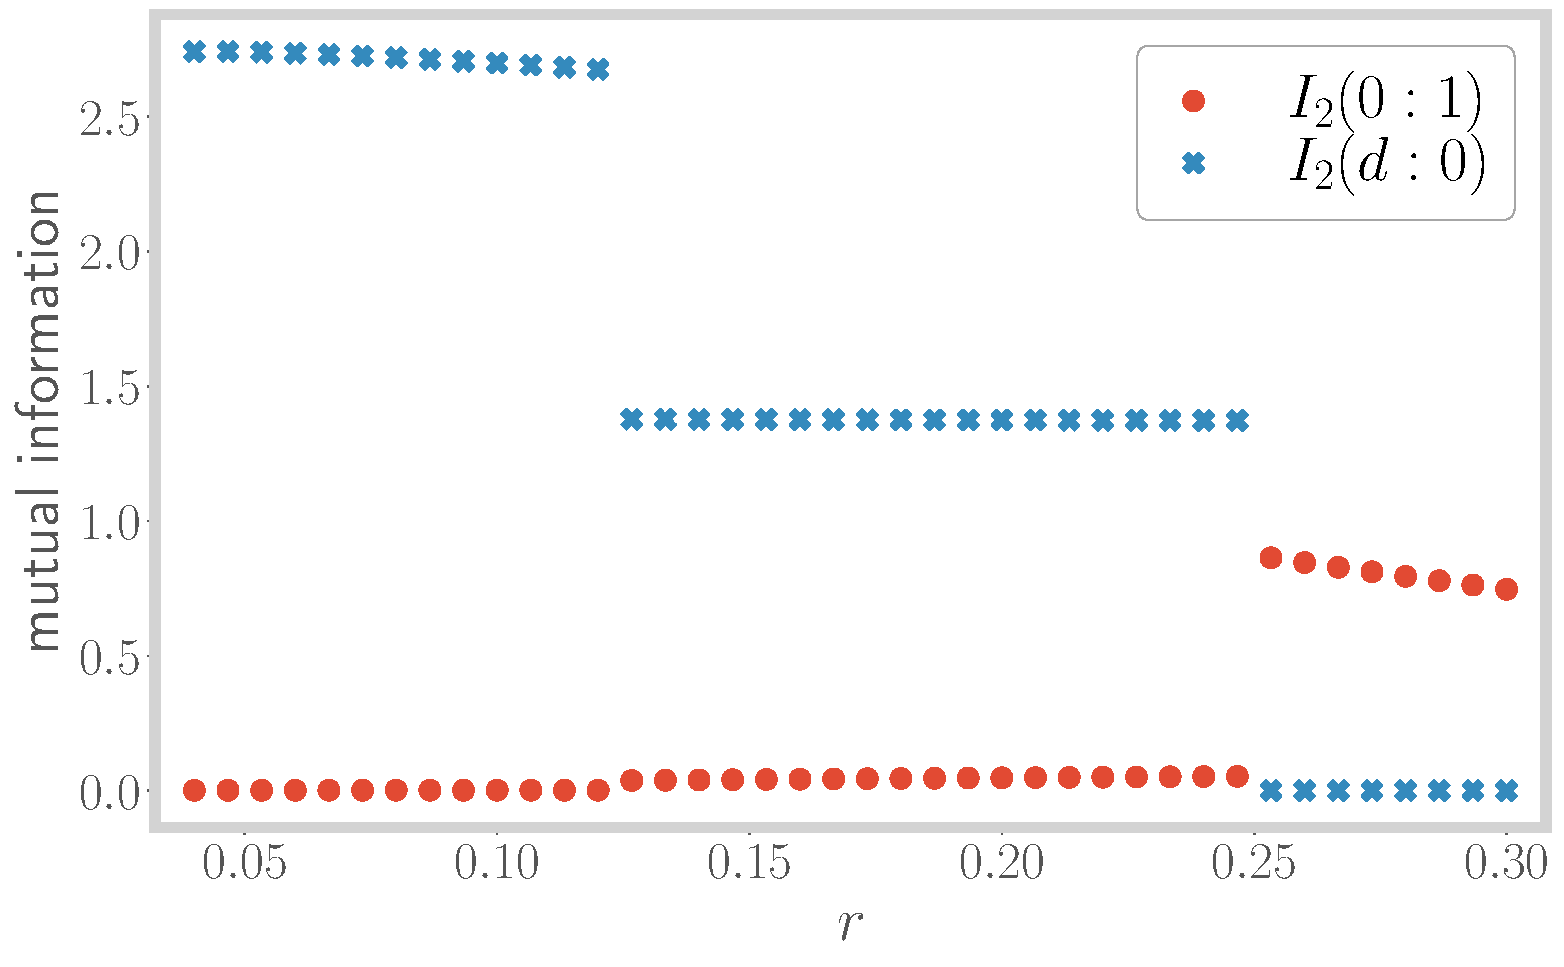
\includegraphics[width=0.4\textwidth]{mutinfo-d0-01-full.pdf}\\
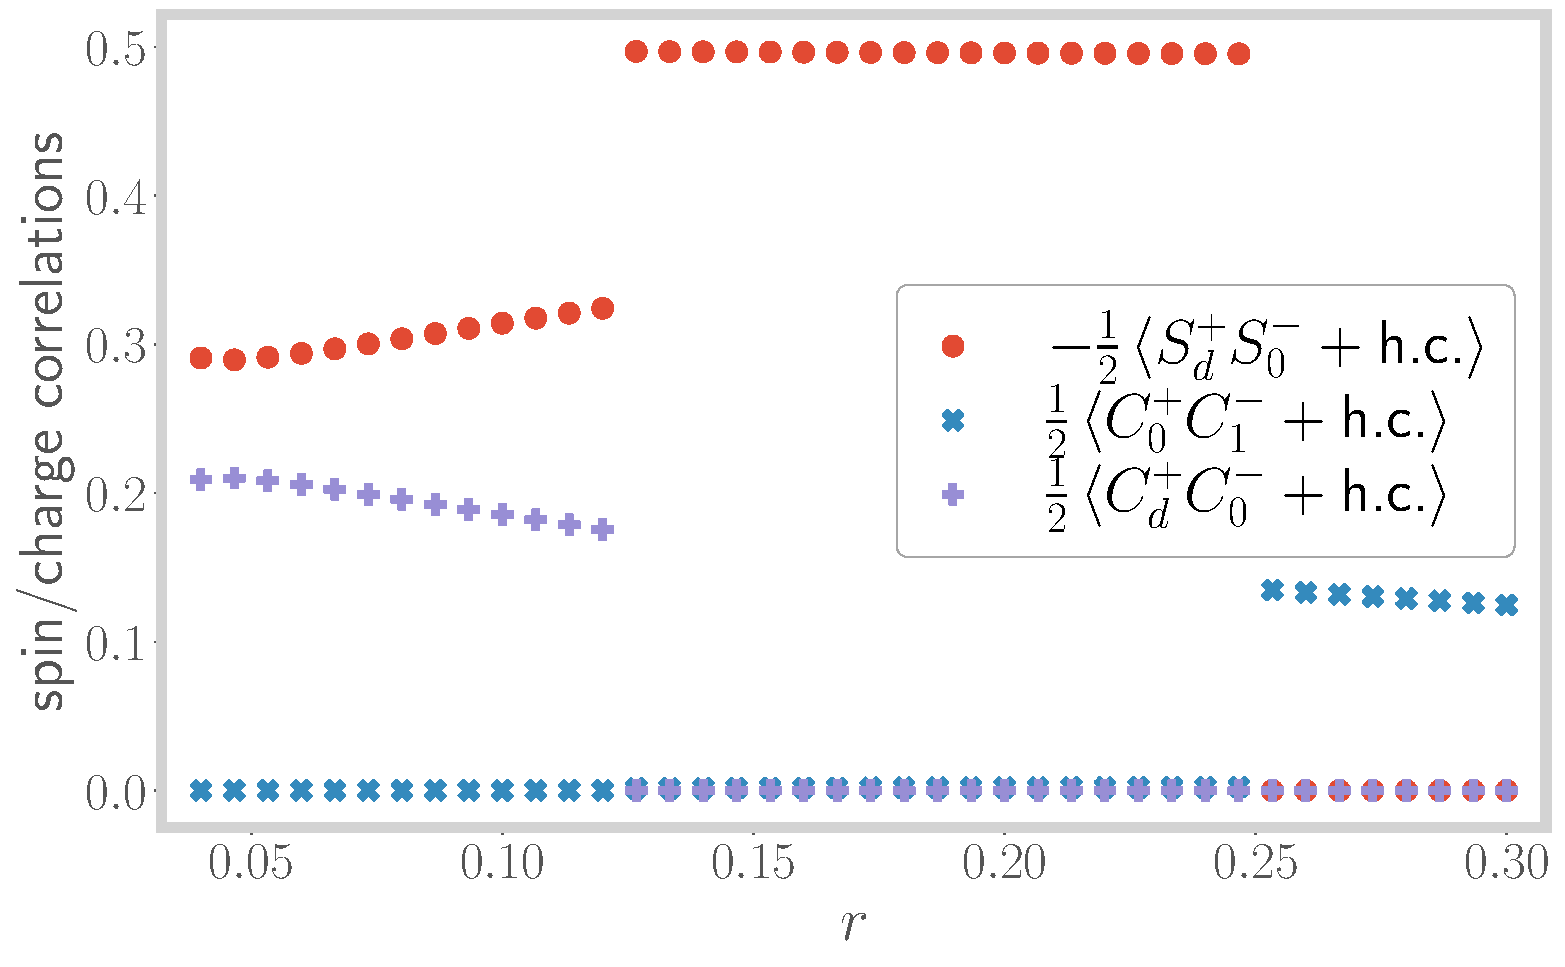
\includegraphics[width=0.4\textwidth]{spin-charge-corr-full.pdf}

{\bf Correlations near \(r_{c1}\)}\par\noindent
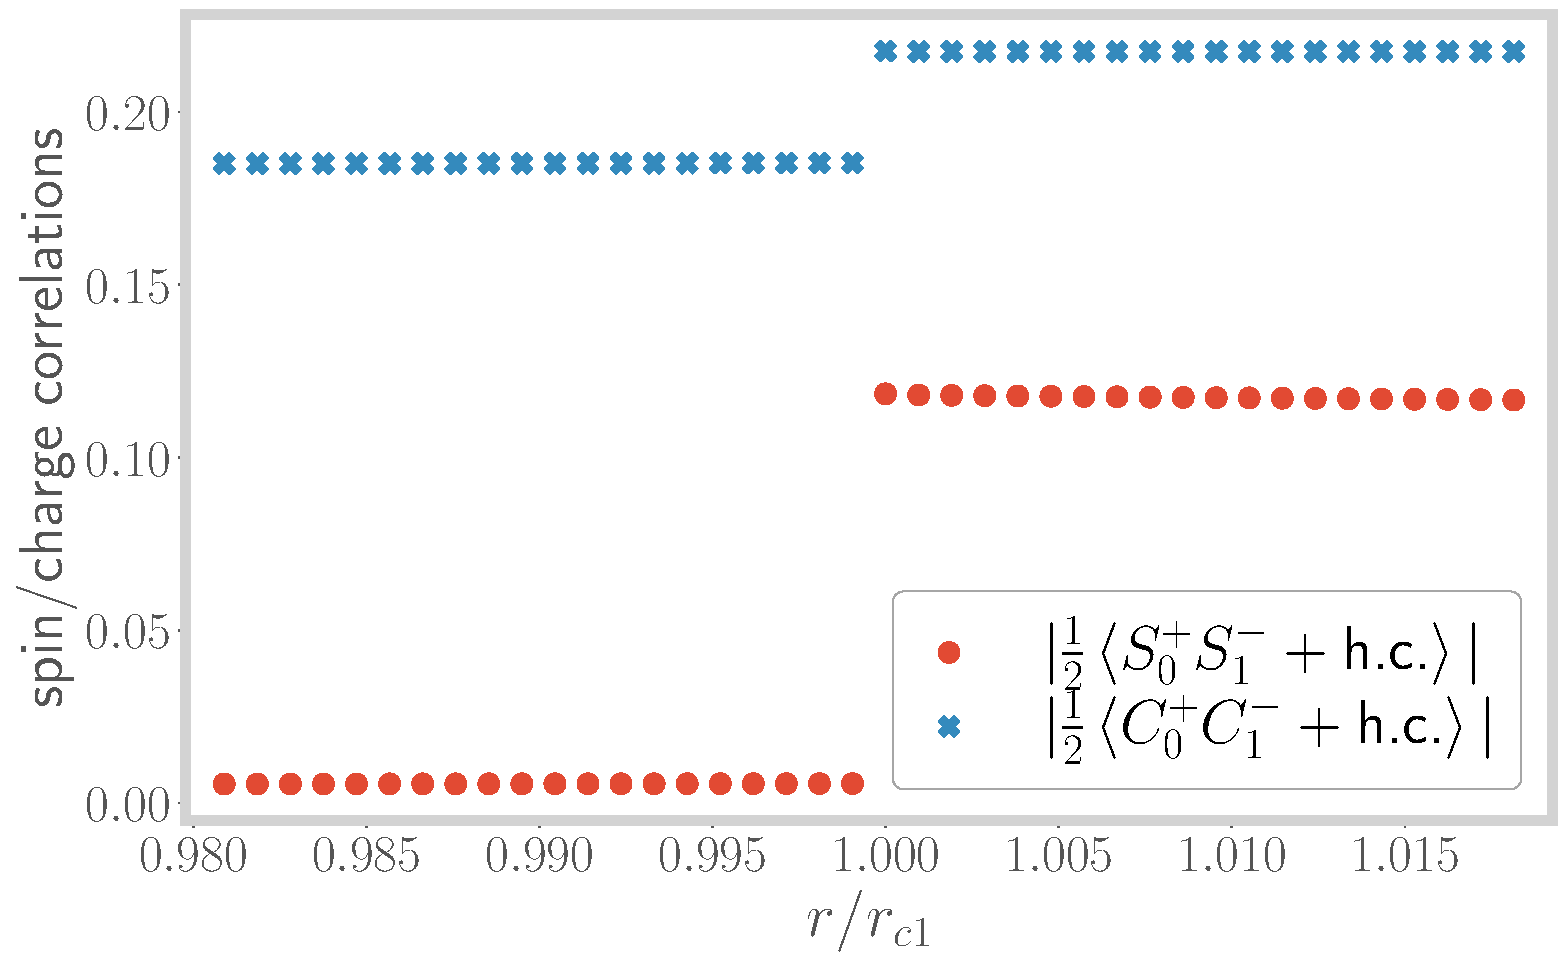
\includegraphics[width=0.4\textwidth]{Uc1-spin-charge-01.pdf}
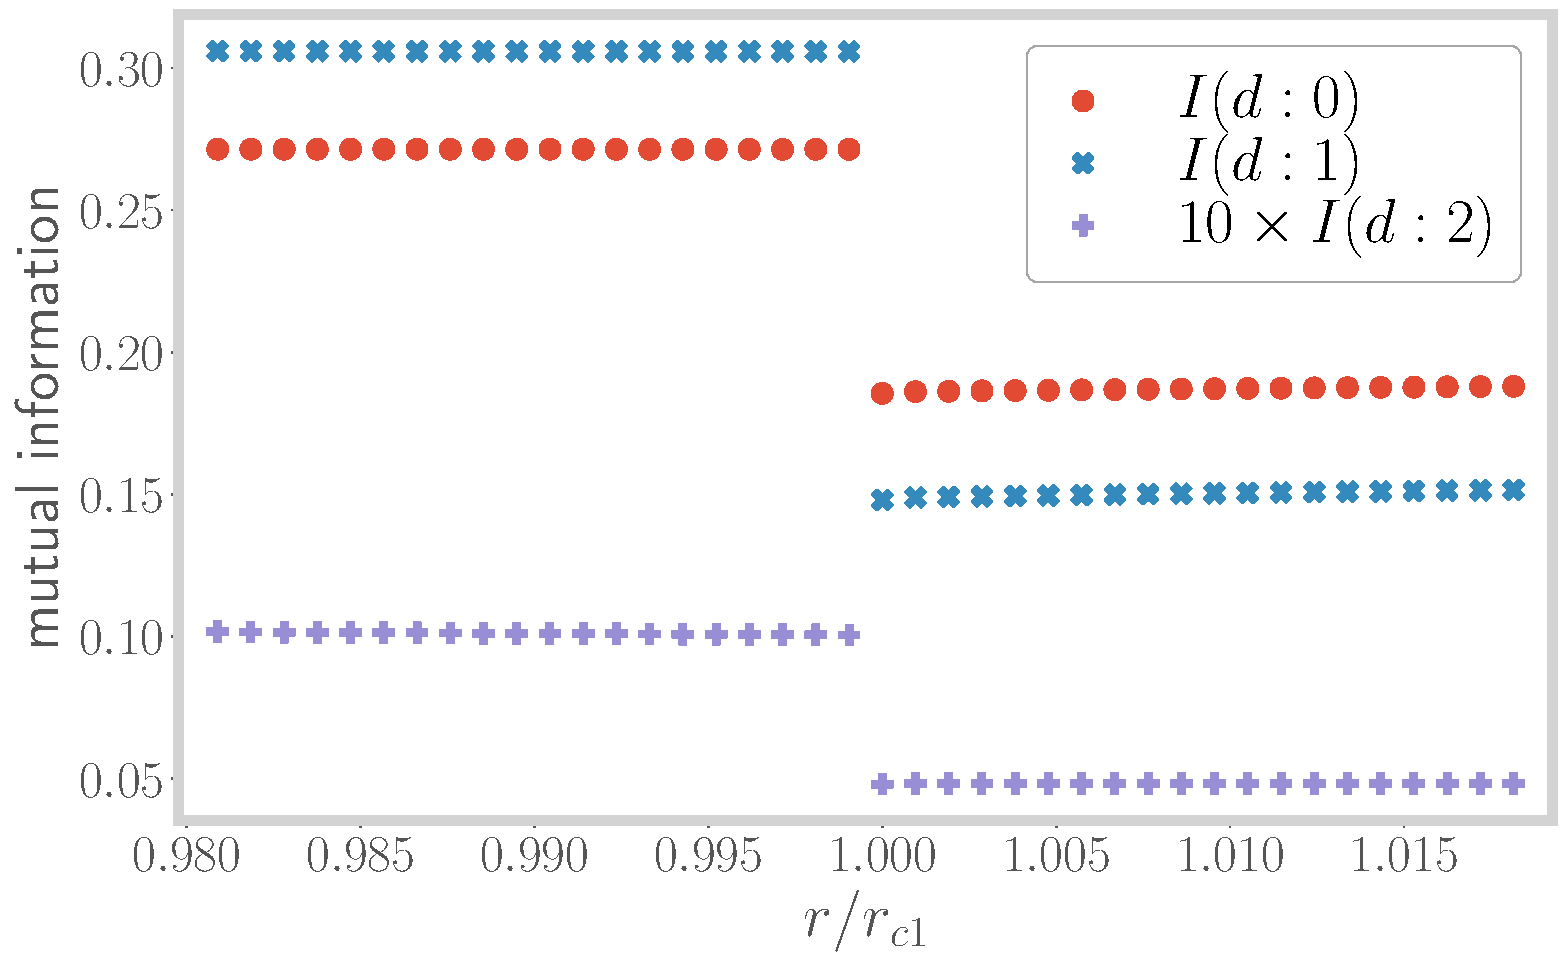
\includegraphics[width=0.4\textwidth]{Uc1-mutinfo.pdf}

{\bf Correlations near \(r_{c2}\)}\par\noindent
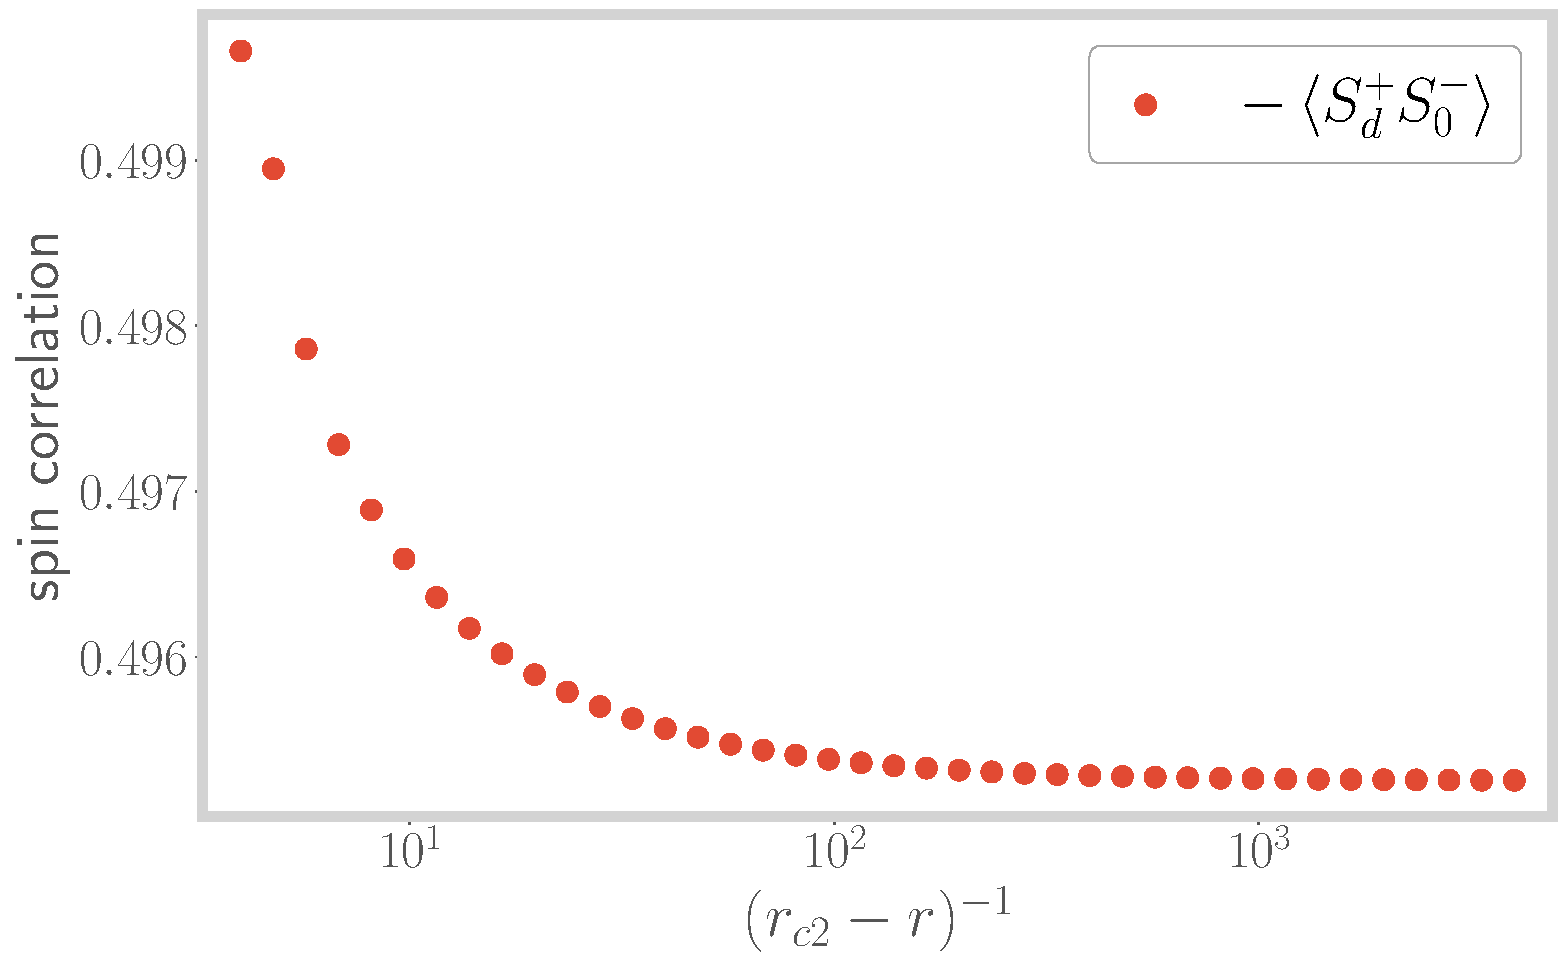
\includegraphics[width=0.4\textwidth]{rc2-spin-corr.pdf}
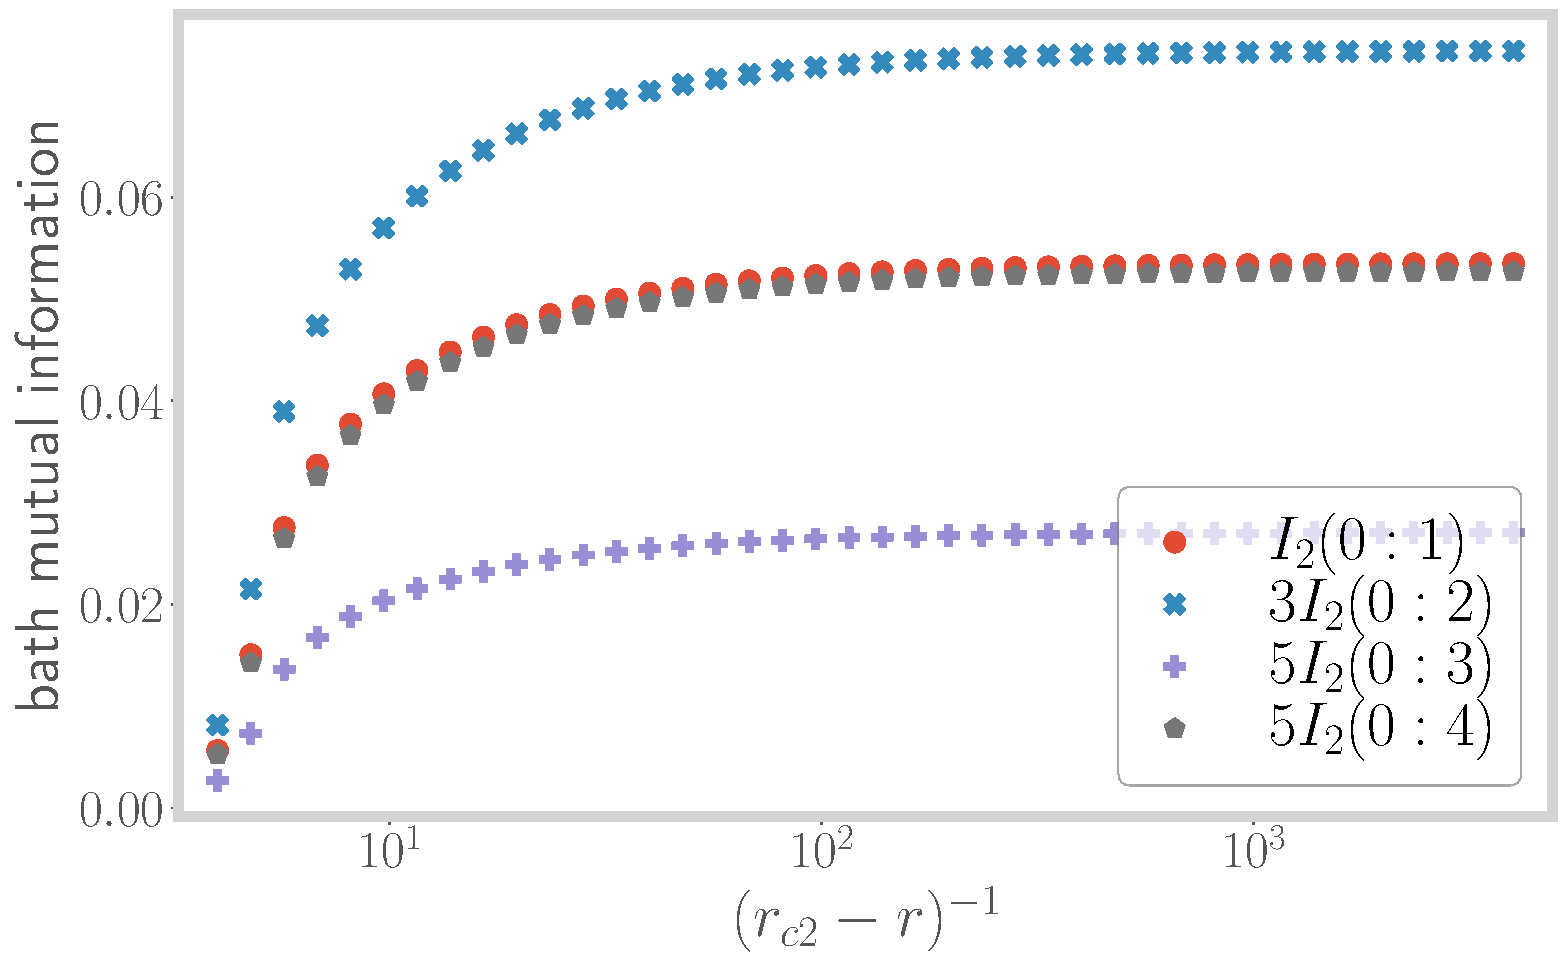
\includegraphics[width=0.4\textwidth]{rc2-mut-info-bath.pdf}\\
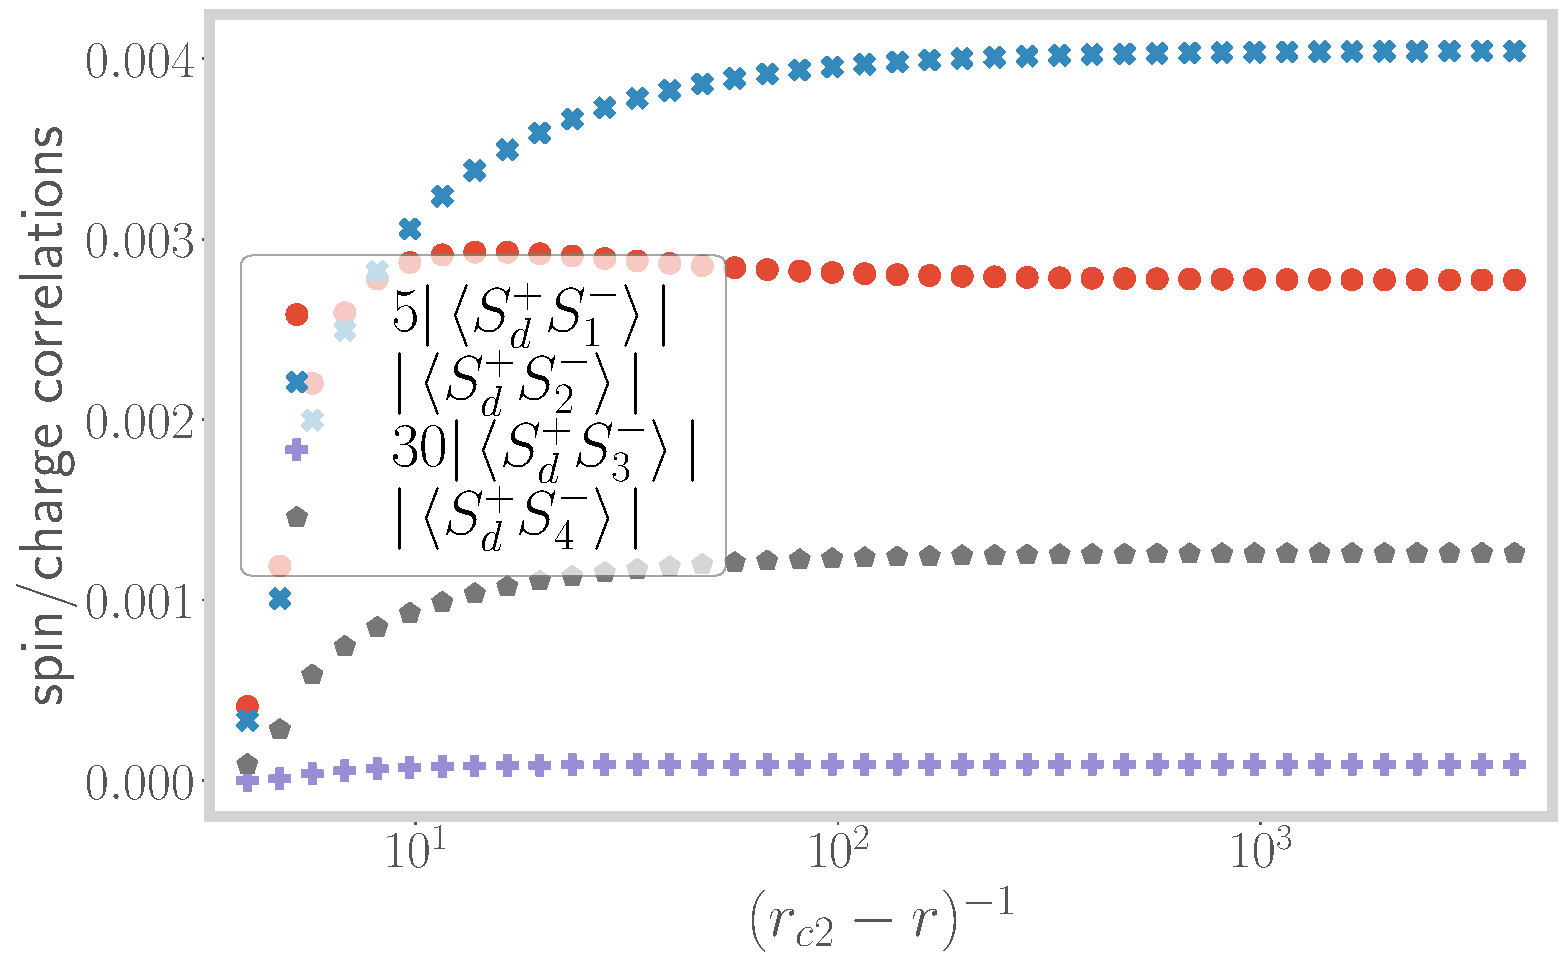
\includegraphics[width=0.4\textwidth]{rc2-spin-flip-di.pdf}

{\bf Correlations about \(r_{c2}\)}\par\noindent
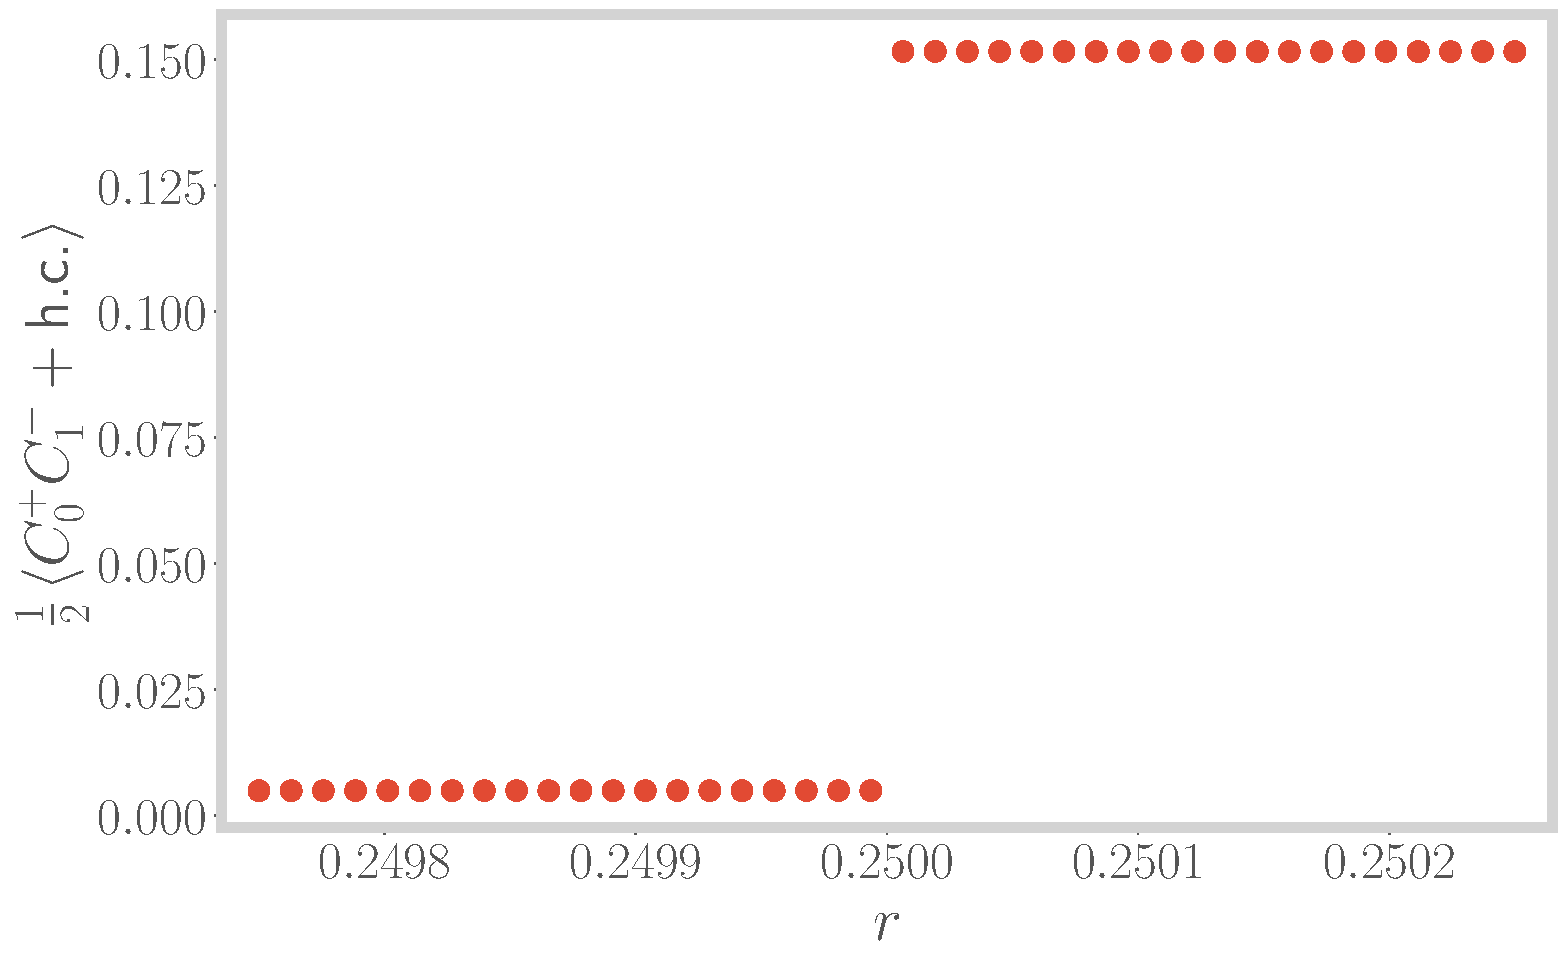
\includegraphics[width=0.4\textwidth]{charge-flip-01-across.pdf}
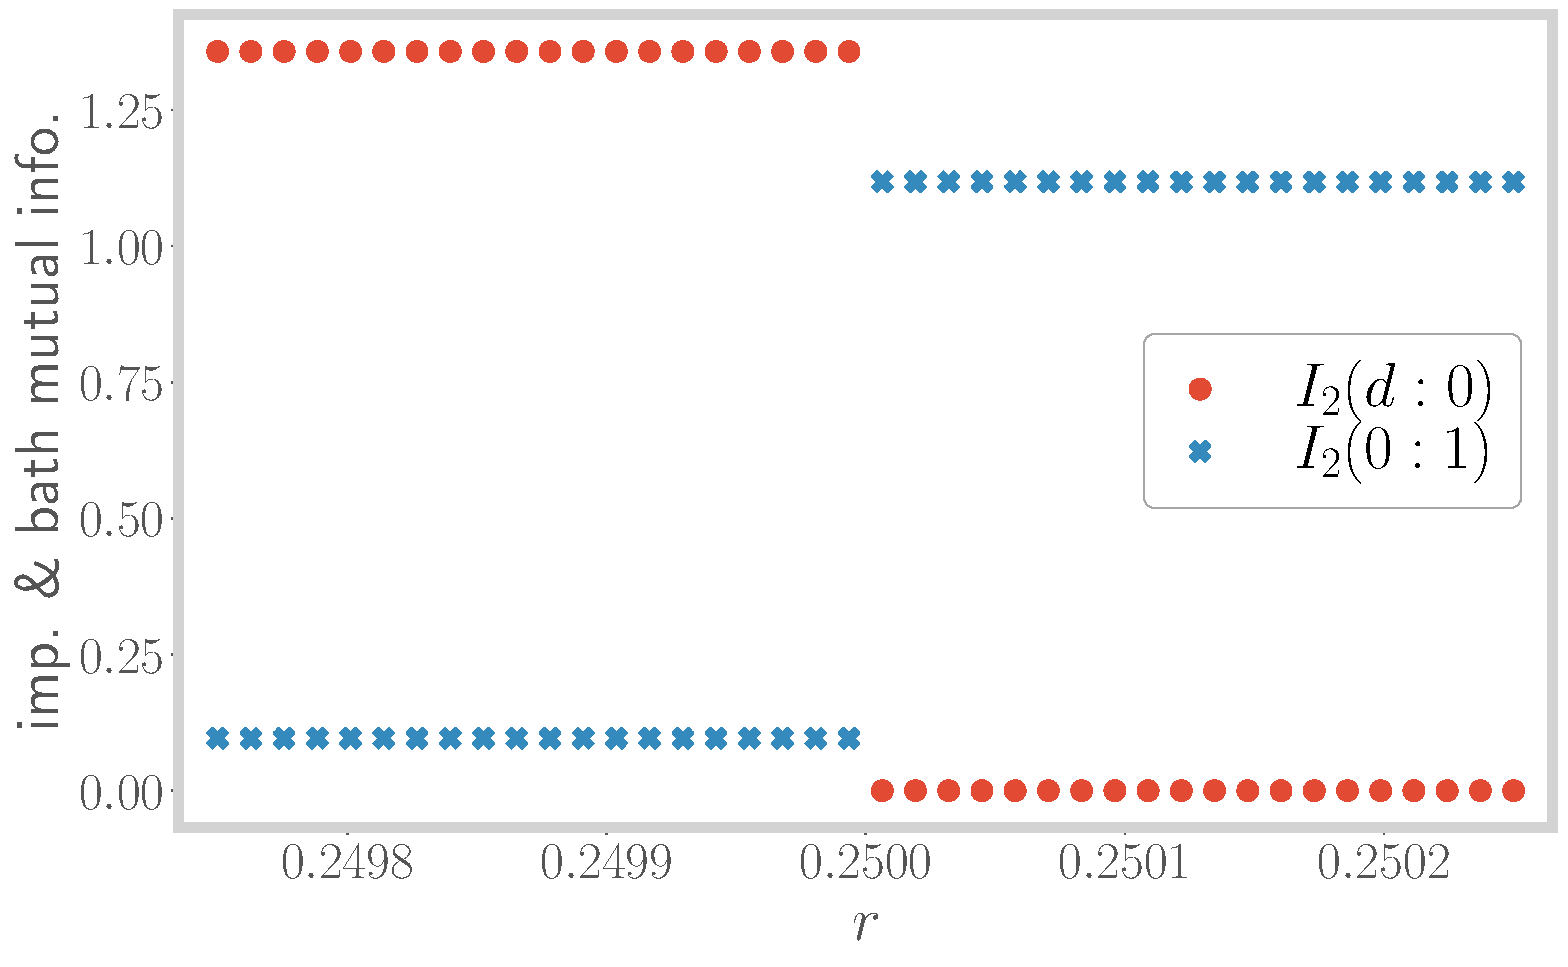
\includegraphics[width=0.4\textwidth]{mut-info-d0-01-across.pdf}

{\bf Analytical expression for \(r_{c1}\)}\par\noindent
For small values of the bare \(J\) (compared to the bandwidth), the irrelevance of \(V\) occurs because of the change in the sign of the denominator \(d_1\). This allows us to obtain an analytical expression for the curve \(r = r_{c1}(J_0/D_0)\). The zero of the denominator \(d_1\) occurs at
\[
	\omega - \frac{D_0}{2} + \frac{U_b}{2} + \frac{U_0}{2} + \frac{J_0}{4} = 0~.
\]
Defining \(f_U = U_0/|U_b|\) and \(f_J = J_0/D_0\) and using the choice \(\omega = -U_0/4 = -f_U|U_b|/4\) allows us to simplify the equation into
\[
	-f_U|U_b|/4 - \frac{J_0}{2f_J} - \frac{|U_b|}{2} + \frac{f_U |U_b|}{2} + \frac{J_0}{4} = 0 \implies \frac{|U_b|}{J_0} \equiv r_{c1} = \frac{2/f_J - 1}{f_U - 2}~.
\]

  

\end{document}

